
\begin{frame}{Background and Motivation}
Many solid breeder designs are now employing a \textbf{breeder unit} configuration
\begin{itemize}
	\item Packed sub-modules of ceramic pebble beds
	\item Units individually tested experimentally and qualified during design phase
\end{itemize}

Must understand how packing states may evolve from time-dependent phenomena (\text{e.g.} pebble damage from crushing, sintering, creep, etc.)
\begin{itemize}
	\item Decrease in effective thermal conductivity raises bed temperatures
	\item Pebble isolation creating hot spots and sintering -- potentially decreasing tritium release rates
\item Gap formation decreases interfacial heat conductance and leads to neutron streaming, etc.
\end{itemize}

\end{frame}

\begin{frame}
\begin{figure}
	\centering
	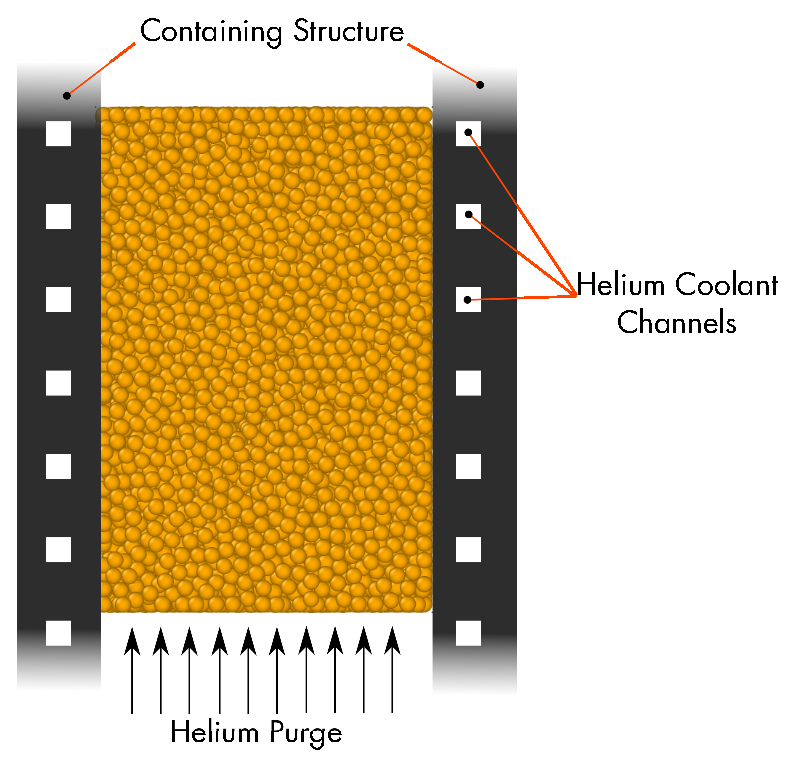
\includegraphics[width=0.85\textwidth]{chapters/figures/solid_breeder_sketch} 
	\caption{Sketch of a typical unit of a pebble bed tritium breeding zone. The pebble bed is cooled with contact to the containing structure.}
	\label{fig:solid-breeder-sketch}
\end{figure}
\end{frame}

\begin{frame}{Modeling Techniques}
\begin{block}{Discrete element method}
Particle-scale information of forces and temperatures for modeling and predicting pebble damage
\end{block}
\begin{block}{Coupled computational fluid dynamics and discrete element method}
Volume-averaging fluid flow for efficient simulations of large volumes with transient, coupled modeling to pebble-scale DEM computations
\end{block}
\begin{block}{Lattice-Boltzmann method}
Interrogate the entire, tortuous flow path with efficient modeling of fluid flow through geometrically complex packing structures
\end{block}
\end{frame}